\chapter{Project Goals}\label{ch:goals}

\section{Overview}

An overview of the project goal definition document is presented below. The different sections which compose it are the following:

\begin{itemize}
\item \textbf{Project definition:} Statement of the goals of the project, specification of its functional aspects and scope.
\item \textbf{Final product:} Description of the products that are to be developed on the project.
\item \textbf{Project realization:} Definition of the different activities to be carried out in order to fulfill the goals of the project.
\item \textbf{Organization and team:} Description of the Work Team that will carry out the project, as well as its organizational structure and human resources plan.
\item \textbf{Execution conditions:} Project related work conditions, definition of the criteria over which product reception as well as the Change Control.
\item \textbf{Planning:} Establishing of the phases and tasks needed to carry the project, together with orientative dates for their realization.
\item \textbf{Project budget:} Determination of the budget of the project and the associate costs.
\end{itemize}

\section{Project definition}

\subsection{Goals}

The main goal of this project is the combination of geospatial and semantic technologies to build a location aware service based on linked data principles.

The main purpose of the service is to provide the users the capacity to share their knowledge in form of routes and points of interest and to enrich the information obtained using data from the web. Then the generated knowledge can be used to recommend the users new routes or points of interests based on their location and preferences.

The knowledge obtained on the system will be published following the Linked Open Data best practices, so that it can be used by other developers or interested groups.

In addition, it will be possible to obtain an objective difficulty rating for the routes or trails that the users share in the system, relieving from the users the problem of rating their own routes and eliminating possible subjective interpretations.

Together with this, several other services will be provided, allowing users to follow trails from others, to post notes at certain location and to obtain in any moment information regarding their surroundings; all in order to build a GPS community around this service.

So, in short, the goals of the project can be stated in the following way:

\begin{itemize}
\item To build a semantic location-aware service
\item To publish the data of the system following the pattern of Linked Open Data
\item To create a model for the semantic representation of trails and points of interest
\item To build a service that allows the correction and evaluation of a route
\item To build a GPS community based on the location-aware service
\end{itemize}

\subsection{Scope of the project}

In order to fulfill the stated goals, a GIS system based on semantic data will be built. The scope of the project is limited to the following:

\begin{itemize}
\item Research over the areas, technologies and standards that the project touches.
\item Design of a model for the semantic representation of trails and points of interest and a infrastructure that uses and supports this model.
\item Development of a service that makes use of the researched technologies and standards and that follows the previously created design.
\end{itemize}

\subsubsection*{Scope of the research}

Research will be carried over several topics, listed below in order of relevance:

\begin{itemize}
\item The Semantic Web
\item Linked Open Data
\item GIS
\item GPS devices
\item Geographic information standards
\item Development tools and platforms
\item Similar systems
\end{itemize}

\subsubsection*{Scope of the development}

The design and development will cover the following issues:

\begin{itemize}
\item Design and creation of a semantic ontology
\item Development of a location aware web service 
\item Creation of a web application to access the service
\item Development of a mobile application to complement the web
\item Extraction of data from third party sources on the web 
\end{itemize}

\section{Final product}

The project will result in a GIS system which relies on a semantic back end, that is, it stores the data on RDF format and is able to reason over it. The system will be composed by a server, a web client and a mobile application.

This section describes the characteristics of the products that will compose the system.

\subsection{Server}

The server will be formed by two main components, a semantic data store and a web server. The web server will expose the a endpoint that allows direct read-only access to the database, so that other developers are able to query it. In addition, the server will have a NoSQL database used to store sensible information about the users of the system, with the purpose of providing secure authentication.

\subsubsection*{Semantic data store}

The main function of this component will be the storage of the information existing on the system. Since semantic databases - called triplestore because they store the data using a data structure called triples - use ontology oriented data modeling (see section \ref{sec:owl}), the knowledge kept will not belong solely to domain related data, but will also include a ontology that represents the schema of the database and the relations among the resources.

This data store will be accessed through the HTTP protocol, even locally. In fact, it will be possible to query the data base through a read-only endpoint, accessible using HTTP. This way, any developer will be able to use the data in their application directly, without having to follow any predetermined access functions.

Besides, the component will be complemented by a reasoner. This reasoner will be able to infer new knowledge from the existing one. In this context, this means that it will be able to analyze the statements in the database and using the ontology as a basis it will be able to produce new statements.

In addition to regular reasoning, it will also be possible to reason spatially over the data. This way, it will be possible to use the spatial representations of resources in the system to make spatial queries, based on distance and geometric relations.

\subsubsection*{Web server}

The web server is the component that will contain most of the functionality of the server. First, it will implement most of the functions encountered in typical web systems, including user authentication, media upload and read, create and modify operations. All these functions will be exposed through a API, following the REST style.

In addition to these basic functionality, the server will also be in charge of receiving the information about trails and points of interest and analyzing it to obtain additional data. This includes applying a mathematical method to calculate a difficulty score for trails.

The API will also expose function allowing spatial queries without any need of previous knowledge or expertise on this area. For example, a function will allow asking for all the points of interest at a certain distance from another feature. This queries will be limited to retrieval of routes, points of interest and geolocated notes.

The spatial information that the API provides will be exposed following the GeoJSON format.

The server will communicate with the data store using an HTTP interface and sending SPARQL queries for managing the data. In addition to this, the server will carry the task of analyzing the profile of each user and recommending routes that can interest them.

In addition to the mentioned functionality, the server will also expose a HTML5 web socket based API that the mobile application will use to provide real time services to the users.

\subsection{Web application}

The web application will be the main interface through which the users will be able to access the service. The web application will be developed taking into account that it will have to be visualized correctly in all kind of devices and that minimum loading times are desired.

The client will allow users to upload routes and points of interest from GPX files, a standard format for the interchange of GPS information (see section \ref{sec:gpx}). In addition, user will also be allowed to draw the routes on a map or mark the points of interest.

It will be possible to search information about the different features and users of the system, taking advantage of the semantic data, which allows to easily build search engines which go beyond the classic keyword search. The application will offer a detailed view of the data and the possibility to comment on the different user generated features. All this information is to be presented in a easy to read format, that is, using interactive maps to show geographical information.

In addition to all of these, the web will provide a interactive map of the world. Moving and zooming this map will show the different routes and points of interest that the current view of the map covers, this way it will be possible to explore the data on the system without the need of a text search.

A exclusive functionality that the client will offer is a interactive editor. This editor will allow drawing trails and points of interest, providing a way to share knowledge without the need of a file recorded from a GPS. In addition, it will be possible to edit existing routes or trails imported from a file, providing the users with a way of correcting possible GPS generated errors.

The editor will allow the following functions:

\begin{description}
\item[Draw a route on the map:] By repeatedly clicking on the map, specifying the coordinates which form the trail, the users will be able to generate data without a need of GPX files, however, it will be impossible to analyze this trails due to the lack of altitude data.

\item[Mark a point of interest in the map:] With a single click on the map, it will be possible to mark a point of interest in the specified point. The user will be prompted with a form, and by filling it, the point of interest will be uploaded to the server.

\item[Edit a existing route:] Whether it is downloaded from the platform or imported from a file, it will be possible to edit the coordinates of a route by dragging the points that form it.

\item[Fusing two routes:] It will be possible to join the end of a route with the start of another to create a new route.
\end{description}

\subsection{Mobile application}

The mobile application will provide the users with a mean of viewing and browsing though the data on the system, in a similar manner to the web client. However, many of the functions present on the browser base client, for example the editor, will no be present on the mobile client, for the web application will be designed to be usable in mobile browsers.

In addition to the basic functionality, this component will allow the users to record their own trail as they traverse it using the GPS on the mobile device. It will be possible to upload this record to the server or to export it as a GPX or GeoJSON.

The application will also provide a function that allows user to receive real time notifications about the nearby points of interest and geolocated notes. These features will be filtered according to the user preferences, before notifying the user.

It will also be possible to follow the trails that another user has shared, with the mobile application sending a notification to the person using it every time that he/she deviates to much from the established route and indicating how to correct its trajectory.

Finally, the application will allow the creation of geolocated notes. To do this, the user will simply need to write a text, take a photo or record a video and after specifying some privacy settings, the note will be recorded in the system on the current coordinates of the user.

\section{Project realization}

\subsection{Realization methodology}

The development method to be followed through the project consists on a prototype based iterative development methodology. This procedure allow to develop a project splitting it into different phases and developing a functional part of the project at each phase. Figure \ref{fig:iterative} shows a graphical conceptualization of this development methodology.

\begin{figure}[ht]
  \centering
  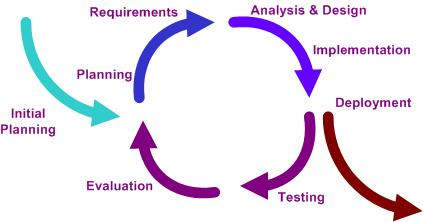
\includegraphics[width=.8\textwidth]{fig/iterative}
  \caption{Iterative development phases}
  \captionsetup{font={footnotesize,bf,it}}
  \caption*{source: \url{http://www.wikipedia.org/}}
  \label{fig:iterative}
\end{figure} 

Thanks to this working methodology, it should be possible to develop independently every components that forms the system and it will be possible to realize effective unit testing over these components.

The development of the project has been split into six phases, whose tasks are listed below. A Work breakdown structure containing the tasks of the project can be found in figure \ref{fig:wbs}.

\subsubsection*{Project opening}
 
This phase consists on the start, organization and planning of the project. The tasks on this phase are not directly related to the development of the final product, yet they are necessary for the development of the project. The tasks in this phase are the following:

\begin{description}
\item[T1.1] Planning and organization

The resources necessary for the realization of the project will be determined and the tasks needed to carry it out will be organized. The development of the project through time will be established.

\item[T1.2] Monitoring

This task will be carried through the whole project. The current status of the project will be monitored to determine the possible existing issues and to ensure that the goals are being reached.
\end{description}

\subsubsection*{Initial research}

The research related with the areas that the project touches will be carried out. The goal of the phase is to obtain the sufficient information to develop a efficient and valid system.

\begin{description}
\item[T2.1] Research on the Semantic Web and Linked Open Data

Research will be done on topics and technologies related to the Semantic Web and Linked Open Data. Other topics will also be investigated, for instance, the representation of spatial data using RDF.

\item[T2.2] Research on technologies

GIS systems, and web and application development tools will be investigated with the goal of establishing an adequate development environment for the project.

\item[T2.3] Analysis of standards and similar system

Existing standards for trail and point of interest representation will be analyzed, as well as the use of this on other platforms and the functionality that similar services offer.

\end{description}

\subsubsection*{Base system development}

The design of the architecture of the system and the development of the software that will be present on the server will be done in this phase. The tasks consist mostly on design, coding and testing.

\begin{description}
\item[T3.1] System design

The technological architecture of the system and of its components will be designed.

\item[T3.2] Test design

The tests to be carried on every component will be determined.

\item[T3.3] Database installation and testing

The semantic database will be installed and tested to guarantee that the desired functionality is granted.

\item[T3.4] Web server implementation and testing

The basic functionality of the web server and related software will be developed and tested. An example of these additional software pieces is the data store connector.

\item[T3.5] API implementation and testing

The functions that the API of the web server exposed will be developed and tested.

\end{description}

\subsubsection*{Web application development}

The web application will be developed using the server produced on the previous phase. Tasks involve mainly interface design, web development and testing.

\begin{description}
\item[T4.1] Interface design

The design of the web interface will be done and the needed resources, such as images and fonts, will be obtained.

\item[T4.2] Implementation and testing

The logic on the web application will be coded and test will be carried out over the developed functions.

\item[T4.3] Editor implementation and testing

The functionality regarding the map editor will be developed and tested.
\end{description}

\subsubsection*{Mobile application development}

The mobile application will be developed using the API of the produced server . Tasks involve mainly interface design, HTML5 development and testing.

\begin{description}
\item[T5.1] Interface design

The design of the mobile interface will be done and the needed resources, such as images and fonts, will be obtained.

\item[T5.2] Implementation and testing

The logic on the mobile application will be coded and test will be carried out over the developed functions.

\end{description}

\subsubsection*{Project finalization}

The last phase will take care of the tasks related to project closure and deployment.

\begin{description}
\item[T6.1] System deployment

The web server will be deployed to a accessible URL and the mobile application will be published on the corresponding markets.

\item[T6.2] Project closure

A final check of the completed goals will be done, future lines of work and possible upgrades will be established and the project will be closed.
\end{description}

\begin{figure}[ht]
  \centering
  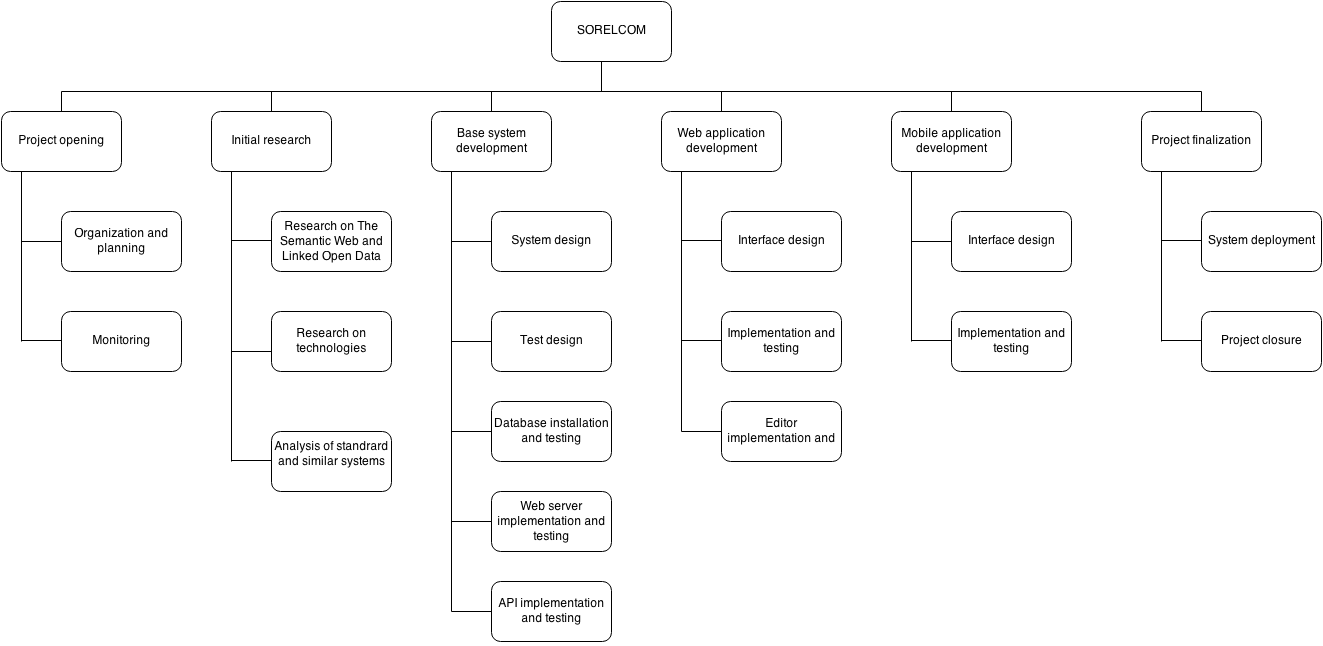
\includegraphics[angle=270, width=.5\textwidth]{fig/wbs}
  \caption{Work breakdown structure}
  \captionsetup{font={footnotesize,bf,it}}
  \label{fig:wbs}
\end{figure} 

\subsection{Intermediate products}

The project is divided on several phases. An intermediate product is obtained from each of the phases or tasks. Table \ref{tab:intermediate-products} offers a reference of the intermediate products of the project and the tasks or phases they relate to.

\begin{table}[ht]
  \centering
  \caption{Intermediate products of the project.}\label{tab:intermediate-products}
  \begin{tabular}{lll}
    \toprule
      \textbf{Name} & \emph{phase}  & \emph{task code}\\
    \midrule
      Technological research & 2. Initial research & T1.1, T1.2 \\
      Ontology specification & 3. Base system development & T3.1 \\
      System architecture & 3. Base system development & T3.1 \\
      Design of the web server & 3. Base system development & T3.1 \\
      Design of the web application & 3. Base system development & T3.1 \\
      Design of the mobile application & 3. Base system development & T3.1 \\
      Test suit & 3. Base system development & T3.2 \\
      Design of the web application interface & 4. Web application development & T4.1 \\
      Design of the mobile application interface & 5. Mobile application development & T5.1 \\
    \bottomrule
  \end{tabular}
\end{table}

These intermediate products are all documents, their contents are listed below:

\begin{description}
\item[Technological research:] Contains a list and of the main technologies that will be involved in the project and a description for each of them.
\item[Ontology specification:] Describes the classes, properties and relations that will appear on the ontology and how they are used to model the data on the system.
\item[System architecture:] Defines which are the components that form the system and how they are related among them.
\item[Design of the web server:] Describes the logical architecture of the web server.
\item[Design of the web application:] Describes the logical architecture of the web application.
\item[Design of the mobile application:] Describes the logical architecture of the mobile application.
\item[Test suite:] Describes the tests to be carried on each of the components of the system.
\item[Design of the web application interface:] Describes the appearance of the web interface.
\item[Design of the mobile application interface:] Describes the appearance of the mobile interface.
\end{description}

\section{Organization and team}

\subsection{Organizational structure}

The organizational structure is relatively simple. The organization involves two main groups, the project manager and the work team.

The project manager is the one in charge of the organization of the project and his function is the direction of the work to do. It takes care of the monitoring and planning of the work as well as most of the validations.

The work group carries out the tasks related to the development of the products of the project. This tasks require research, designs, testing and implementation. The work group will be formed by a single student performing all the required roles.

The organizational schema including all the roles on the project is presented in figure \ref{fig:organization}.

\begin{figure}[ht]
  \centering
  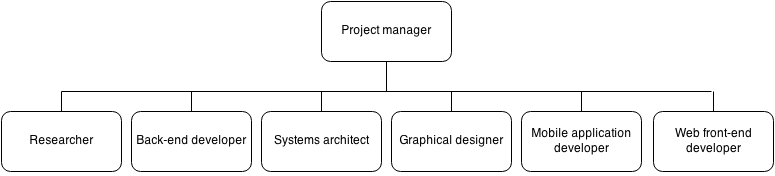
\includegraphics[width=.7\textwidth]{fig/organization}
  \caption{Organizational structure}
  \captionsetup{font={footnotesize,bf,it}}
  \label{fig:organization}
\end{figure} 

\subsection{Human resources plan}

The organization will be formed by the following profiles, each related to the different areas of competence that this project comprises.

\subsubsection*{Project manager}

The project manager is the person in charge of the opening, organization, monitoring and closure of the project. In addition, it is the person in charge of communicating with the management team.

The skills of the project manager should include at least the following:

\begin{itemize}
\item Planning
\item Organizing
\item Communication
\end{itemize}

In addition, it is convenient for it to have knowledge on the areas that the project touches.

\subsubsection*{Researcher}

Due to the innovative nature of the project and the amount of work related to the semantic web, the profile of a researcher is required. The researches takes care of investigating the current state in the areas that the project touches and elaborating state of the art documents needed for the development of the project.

The researcher needs to have knowledge on the areas related to the project, that is, The Semantic Web and Linked Open Data. Learning and writing capabilities are also convenient.

\subsubsection*{Back-end developer}

This profile takes care of developing the back-end of the application, the web server. Due to the nature of its work and the technologies to be used in the project, the following knowledge is required.

\begin{itemize}
\item JavaScript programming skills
\item Knowledge of the NodeJS programming environment
\item Knowledge of the SPARQL query language
\end{itemize}

\subsubsection*{Front-end web developer}

The web developer takes care of creating the web application. Its work involves development of web based graphical user interfaces, due to this and the technologies chosen for the project, the following skills are required.

\begin{itemize}
\item HTML5, CSS3 and JavaScript
\item The AngularJS web development framework
\item The CSS framework Twitter Bootstrap
\item The JavaScript map development library Leaflet
\end{itemize}

\subsubsection*{Mobile application developer}

This profile takes care of developing the mobile application. Proficiency on mobile application programming is needed, however, it is also necessary to know how to use HTML5 native development tools. The required skills can be summarized in the following:

\begin{itemize}
\item HTML5, CSS3 and JavaScript
\item The HTML5 web sockets protocol
\item The HTML5 native mobile development library Phonegap
\item The JavaScript map development library Leaflet
\end{itemize}

\subsubsection{Graphical designer}

The graphics designer takes care of designing the interface of the application. In order to present this design it is required that the designer knows how to use some graphic design tool such as GIMP or Photoshop. 

\subsubsection{Systems architect}

The systems architect takes care of designing the system architecture and the logical design of each component. It should have the following skills:

\begin{itemize}
\item Software design
\item The modeling standard UML
\end{itemize}

\section{Execution conditions}

The usual workplace will be the DeustoTech office located in the 4th floor of the ESIDE building in the university of Deusto. In this environment ethernet network connection is provided as well as a power source for computers. Still, a personal laptop is to be used for the development instead of office computer. Mobile devices used for testing will also be properties of the student.

The weekly schedule is of 18 hours, divided in three hours per day. 

\subsection{Hardware}

Since web and mobile applications are to be developed, there is a need to carry out tests and preview results in various kind of devices, such as mobile phones and tablets. The hardware that is available is the following:

\begin{itemize}
\item Laptop computer, Inter i7 processor, 15 inch screen
\item Android Smartphone, Nexus 5 model
\item iPad tablet
\end{itemize}

\subsection{Software}

The software tools to be used in the project will be open source in most cases, and just free in the rest. In this section the software that is available is listed:

\subsubsection*{Programming tools}

\begin{itemize}
\item NodeJS 0.10.25 - JavaScript runtime environment
\item NPM 1.3.10 - NodeJS package manager
\item Bower 1.3.3 - JavaScript library management tool
\item Yeoman 1.1.2 - JavaScript project scaffolding tool
\item Express 3.4.3 - NodeJS web development library
\item AngularJs 1.2.11 - JavaScript web application development framework
\item Leaflet 0.7.3 - JavaScript map developing library
\item Twitter Bootstrap 3 - CSS responsive web development framework
\item SASS 3.3.8 - CSS development framework
\item Phonegap 2.9.1 - Mobile HTML5 programming platform
\end{itemize}

\subsubsection*{Web browsers}

\begin{itemize}
\item Google Chrome 27 
\item Mozilla Firefox 22
\item Safari 6
\item Opera 12
\item Internet Explorer 10
\end{itemize}

\subsubsection*{Others}

\begin{itemize}
\item Ubuntu 14.04 - Open source desktop operating system
\item Atom 0.105 - JavaScript based code editor
\item Parliament 2.6 - Semantic spatial database, reasoner and endpoint
\item GIT 2.0.0 - Version control system
\item GIMP 2.8 - Image manipulation program
\end{itemize}

\subsection{Change control}

The changing requirements or petitions will follow the proceeding described below:

\begin{enumerate}
\item The change will be communicated to the work group, in case it comes from outside stakeholders.
\item The work group will study the request and evaluate the impact of the potential change in the project.
\item The work group will produce a report that will be sent to the project manager.
\item The project manager will take the final decision on whether to accept the changes or not.
\end{enumerate}

\subsection{Product reception}

During this project two types of product will be created, documents and software. Both of them will be accepted following different procedures.

The documents will follow a previously determined structure. This structure requires each document to have a index, a figure and table index and a list of references used. There is only one requirement regarding the content, documents must start with a overview of the contents of the paper. The author and title of the document must appear at the beginning.

These documents will be sent to the project manager, who will have to accept it in a period of 5 working days. In case of a lack of response, the work team will assume that the document has been accepted so that the development of the project is not stopped.

The software on the other side will follow more rigorous criteria. On the task \textbf{SYS2}, a document specifying the test suite for each component will be created. Software components will only be accepted when they have passes all the specified tests.

\newpage
\FloatBarrier
\section{Planning}

This section presents several aspects related to the project planning. The planning considers a work schedule of 3 hours each day. The project starts Monday 3 of march 2014 and will end the 10th of July of the same year.

\subsection*{Workload estimation per profile}

The estimated work to be done by each profile is shown on this section. 

Table \ref{tab:manager} contains the work to be done by the project manager.

\begin{table}[ht]
  \centering
  \caption{Workload estimation for the project manager.}\label{tab:manager}
  \begin{tabular}{ll}
    \toprule
      \textbf{Task} & \emph{hours}\\
    \midrule
      T1.1 & 6\\
      T1.2 & 16\\
      T6.2 & 3\\
    \bottomrule
      \textbf{Total} & 25\\
  \end{tabular}
\end{table}

Table \ref{tab:architect} contains the work to be done by the system architect.

\begin{table}[ht]
  \centering
  \caption{Workload estimation for the system architect.}\label{tab:architect}
  \begin{tabular}{ll}
    \toprule
      \textbf{Task} & \emph{hours}\\
    \midrule
      T3.1 & 45\\
      T3.2 & 6\\
    \bottomrule
      \textbf{Total} & 51\\
  \end{tabular}
\end{table}

Table \ref{tab:researcher} contains the work to be done by the researcher.

\begin{table}[ht]
  \centering
  \caption{Workload estimation for the researcher.}\label{tab:researcher}
  \begin{tabular}{ll}
    \toprule
      \textbf{Task} & \emph{hours}\\
    \midrule
      T2.1 & 15\\
      T2.2 & 12\\
      T2.3 & 15\\
    \bottomrule
      \textbf{Total} & 42\\
  \end{tabular}
\end{table}

Table \ref{tab:backend} contains the work to be done by the back-end developer.

\begin{table}[ht]
  \centering
  \caption{Workload estimation for the back-end developer.}\label{tab:backend}
  \begin{tabular}{ll}
    \toprule
      \textbf{Task} & \emph{hours}\\
    \midrule
      T3.3 & 3\\
      T3.4 & 30\\
      T3.5 & 24\\
      T6.2 & 3\\
    \bottomrule
      \textbf{Total} & 60\\
  \end{tabular}
\end{table}

Table \ref{tab:webdev} contains the work to be done by the front-end web developer.

\begin{table}[ht]
  \centering
  \caption{Workload estimation for the front-end web developer.}\label{tab:webdev}
  \begin{tabular}{ll}
    \toprule
      \textbf{Task} & \emph{hours}\\
    \midrule
      T4.2 & 27\\
      T4.3 & 21\\
    \bottomrule
      \textbf{Total} & 48\\
  \end{tabular}
\end{table}

Table \ref{tab:mobdev} contains the work to be done by the mobile application designer.

\begin{table}[ht]
  \centering
  \caption{Workload estimation for the mobile application developer.}\label{tab:mobdev}
  \begin{tabular}{ll}
    \toprule
      \textbf{Task} & \emph{hours}\\
    \midrule
      T5.2 & 21\\
    \bottomrule
      \textbf{Total} & 21\\
  \end{tabular}
\end{table}

Table \ref{tab:designer} contains the work to be done by the graphics designer.

\begin{table}[ht]
  \centering
  \caption{Workload estimation for the graphics designer.}\label{tab:designer}
  \begin{tabular}{ll}
    \toprule
      \textbf{Task} & \emph{hours}\\
    \midrule
      T4.1 & 12\\
      T5.1 & 9\\
    \bottomrule
      \textbf{Total} & 21\\
  \end{tabular}
\end{table}

\subsection*{Network and Gantt diagram}

Figure \ref{fig:gantt} shows the gantt diagram for the project, which establishes the temporal planning.
Figure \ref{fig:network-diagram} shows the network diagram of the tasks on the project, in order to identify the dependencies among them.

\begin{figure}[ht]
  \centering
  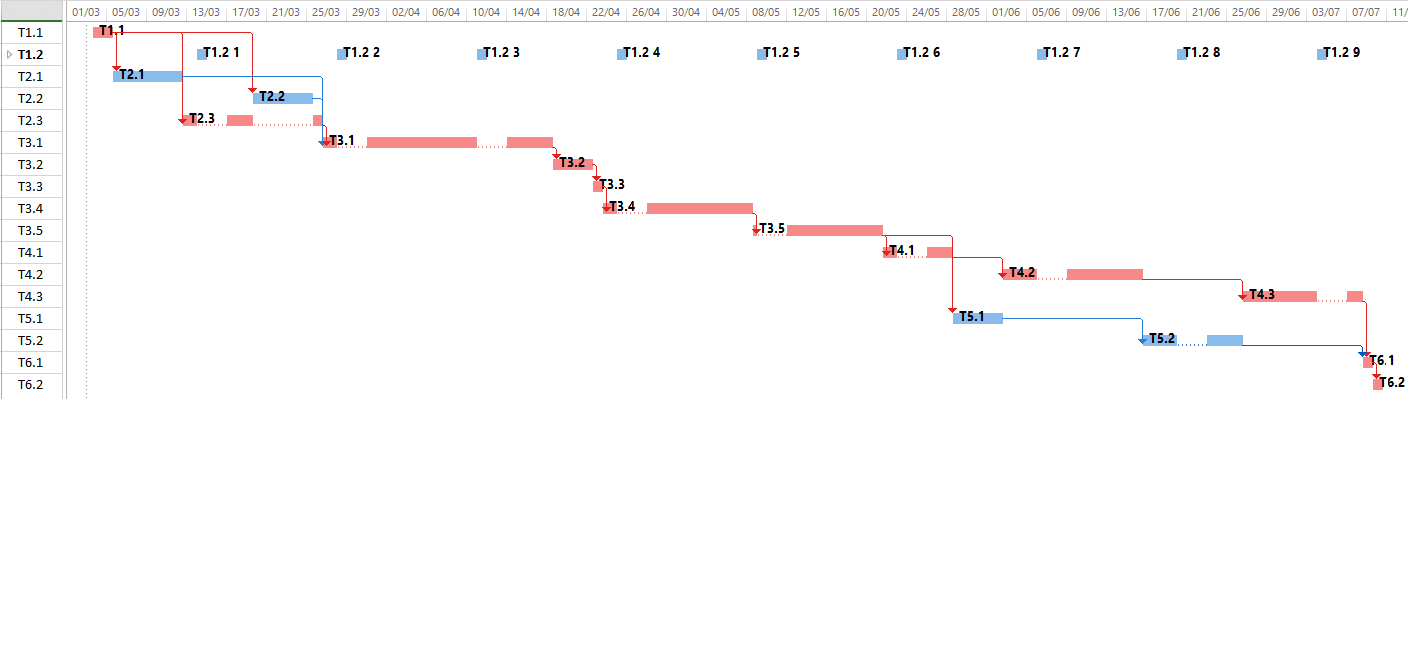
\includegraphics[angle=270,width=.6\textwidth]{fig/gantt-diagram}
  \caption{Gantt diagram}
  \captionsetup{font={footnotesize,bf,it}}
  \label{fig:gantt}
\end{figure} 


\begin{figure}[ht]
  \centering
  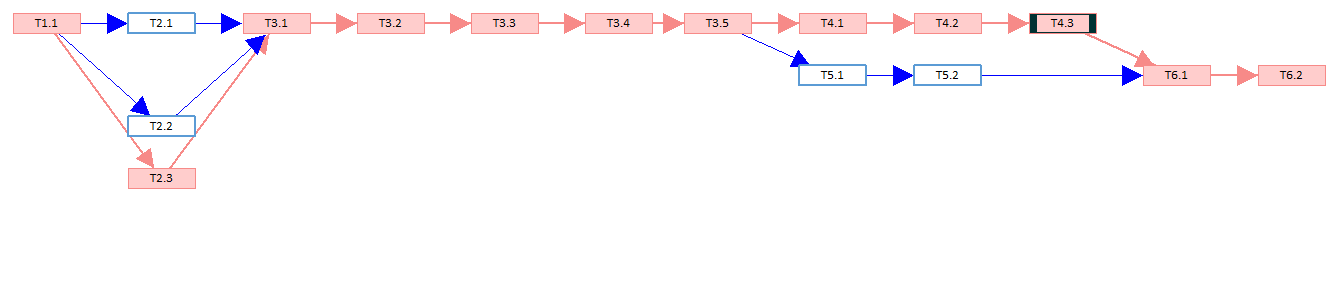
\includegraphics[angle=270, width=.3\textwidth]{fig/network-diagram}
  \caption{Network diagram}
  \captionsetup{font={footnotesize,bf,it}}
  \label{fig:network-diagram}
\end{figure} 

\subsection*{Work plan}

The work plan obtained after establishing the schedule and the interdependencies among tasks is presented in table \ref{tab:project-plan}.

\begin{table}[ht]
  \centering
  \caption{Real work plan.}\label{tab:project-plan}
  \begin{tabular}{llllll}
    \toprule
      \textbf{Identifier} & \emph{start} & \emph{end} & \emph{days} & \emph{profile} & \emph{work (h)}\\
    \midrule
      \textbf{T1 - Project initiation}\\
    \midrule
	  T1.1 & 03/03 & 05/03 & 2 & Project manager & 6\\
      T1.2 & 10/03 & 13/06 & 8 & Project manager & 16\\
    \midrule
      \textbf{T2 - Initial research}\\
    \midrule
      T2.1 & 05/03 & 12/03 & 5 & Researcher & 15\\
      T2.2 & 19/03 & 25/03 & 4 & Researcher & 12\\
      T2.3 & 12/03 & 26/03 & 5 & Researcher & 15\\
    \midrule 
      \textbf{T3 - Base system development}\\
    \midrule
      T3.1 & 26/03 & 18/04 & 15 & System architect & 45\\
      T3.2 & 18/03 & 22/04 & 2 & System architect & 6\\
      T3.3 & 22/04 & 23/04 & 1 & Back-end developer & 3\\
      T3.4 & 23/04 & 08/05 & 10& Back-end developer & 30\\
      T3.5 & 08/05 & 21/05 & 8 & Back-end developer & 24\\
    \midrule
      \textbf{T4 - Web app. development}\\
    \midrule
      T4.1 & 21/05 & 28/05 & 4 & Graphics designer & 12\\
      T4.2 & 02/06 & 16/06 & 9 & Front-end developer & 27\\
      T4.3 & 26/06 & 08/07 & 7 & Front-end developer & 21\\
    \midrule
      \textbf{T5 - Mobile app. development}\\
    \midrule
      T5.1 & 28/05 & 02/06 & 3 & Graphics designer & 9\\
      T5.2 & 16/06 & 26/06 & 7 & Mobile app developer & 21\\
    \midrule
      \textbf{T6 - Project finalization}\\
    \midrule
      T6.1 & 08/07 & 09/07 & 1 & Back-end developer & 3\\
      T6.2 & 09/07 & 10/07 & 1 & Project manager & 3\\
  \end{tabular}
\end{table}

\newpage
\FloatBarrier
\section{Project budget}

The costs associated with the project are divided into two main sources. The first group is the hardware related costs, which comprises the budget required for the physical technological resources used in the realization of the project. Table \ref{tab:hardware} reflects these costs.

The second cost it the one destined to the human resources team. An overview of the costs generated by each profile may be found in table \ref{tab:hhrr}.

No budget will be destined to cover software cost, for the tools used on the project will all be either open source or free-ware. A summary of the project budget can be found in table \ref{tab:budget}.

\begin{table}[ht]
  \centering
  \caption{Hardware related budget.}\label{tab:hardware}
  \begin{tabular}{llll}
    \toprule
      \textbf{Name} & \emph{units}  & \emph{unit price (\euro)} & \emph{cost (\euro)}\\
    \midrule
      Laptop computer & 1 & 1000.00 & 1000.00\\
	  Android smart phone & 1 & 450.00 & 450.00\\
	  iOS tablet & 1 & 500.00 & 500.00\\
    \bottomrule
      \textbf{Total} & & & 1950.00\\
  \end{tabular}
\end{table}


\begin{table}[ht]
  \centering
  \caption{Human resources budget.}\label{tab:hhrr}
  \begin{tabular}{llll}
    \toprule
      \textbf{Name} & \emph{work (h)} & \emph{cost (\euro)}\\
    \midrule
      Front-end web developer & 48  & 240.00\\
	  Back-end developer & 60 & 300.00 \\
	  Mobile application programmer & 21 & 105.00\\
	  Graphics designer & 21 & 105.00\\
	  Researcher & 42 & 210.00\\
	  System architect & 51 & 255.00\\
      Project manager & 25 & 125.50\\
    \bottomrule
      \textbf{Total} & & 1340.00\\
  \end{tabular}
\end{table}

\begin{table}[ht]
  \centering
  \caption{Summary of budget.}\label{tab:budget}
  \begin{tabular}{llll}
    \toprule
      \textbf{Name} & \emph{cost (\euro)}\\
    \midrule
	  Hardware & 1950.00\\
      Human resources & 1340.00\\
    \bottomrule
      \textbf{Total} & 3290.00\\
  \end{tabular}
\end{table}